\documentclass[spanish]{article}

%%%%%%%%%%%%%%%%%%%%%%%%%%%%%%%%%%%%%%%%%%%%%%%%%%%%%%%%%%%%%%%%%%%%%%%%%%%%%%%%

% Avoiding floating images

% Language
\usepackage[spanish]{babel}

% Support for images
\usepackage{graphicx}

% Underlining
\usepackage{amsmath}

% Avoiding indenting of first paragraph's line.
\setlength{\parindent}{0cm}

% Support for hyperlinks.
\usepackage{hyperref}
\hypersetup {
        linktoc=all,
        hidelinks
}

% Additional section formatting.
\renewcommand\thesection{\arabic{section}}
\renewcommand\thesubsection{\thesection.\arabic{subsection}}

% Cover of the document
\title{Redes y Aplicaciones Internet - Práctica 3}
\author{Oussama Akachach Jouhrati\\
[0.5cm]{\small Profesor/a: Maria Isabel March Hermo}}
\date{\today}

%%%%%%%%%%%%%%%%%%%%%%%%%%%%%%%%%%%%%%%%%%%%%%%%%%%%%%%%%%%%%%%%%%%%%%%%%%%%%%%%

\begin{document}

\pagenumbering{gobble}
\maketitle
\newpage

\tableofcontents
\pagenumbering{arabic}
\setcounter{page}{2}
\newpage


% Customize from here.

\section{Pregunta 1}

\subsection{}

\textit{Explicad todos los parámetros de configuración de
RTMP que habéis añadido en el fichero de configuración
anterior nginx.conf.}\\

El primer parámetro, ``rtmp'' indica el protocolo que
utiliza nuestro servidor. Al ser un servidor de
\textit{streaming}, buscaremos este protocolo de mensajería
en tiempo real.\\

El segundo parámetro, ``server'', contiene la configuración
del servidor. Será donde introduzcamos los parámetros que
llevará nuestro servidor.\\

El tercer parámetro, ``listen'', nos indica el puerto que
está utilizando nuestro servidor.\\

El cuarto parámetro, ``chunk\_size'', nos indica el número de
bytes que tendrá cada paquete o \textit{chunk}, ya que el
mecanismo de transferencia utilizado dividirá los datos en
en paquetes de ese tamaño.\\

El quinto parámetro, ``allow publish all'', da acceso a
publicar contenido a todas las redes.\\

El sexto parámetro, ``application live'', según
digitalocean.com, define un bloque de aplicación que estará
disponible en el path de URL /live.\\

El séptimo parámetro, ``live on'', permite a los usuarios
conectarse a la retransmisión en directo.\\

El octavo y último parámetro, ``record off'', deshabilita la
función de guardado automático de las retransmisiones al
disco duro.

\subsection{}

\textit{Añadid tres parámetros de configuración maś
relacionados con el protocolo RTMP y explicad por qué creéis
interesante tenerlos en cuenta. Mostrad una captura del
fichero nginx.conf dónde aparezcan.}\\

El primer y segundo parámetro que sería interesante
introducir es el que da soporte a protocolos para poder visualizar el
contenido de la retransmisión desde un navegador web,
directamente. Estos serían HLS y MPEG DASH:

\begin{center}
hls on;

dash on;\\
\end{center}

Más adelante, deberíamos añadir configuraciones adicionales
para estos dos protocolos, pero de momento, para los dos
primeros parámetros, establecemos la compatibilidad con
estos dos protocolos.\\

Por último, sería interesante añadir una configuración
adicional para permitir que nuestro retransmisión se pueda
reproducir en otras páginas. Para ello, escribiremos el
siguiente comando, debajo del bloque ``server'':

\begin{center}
allow publish all
\end{center}

\subsection{}

\textit{Para verificar que nginx está funcionando
correctamente, teclead la siguiente orden la consola y
mostrad el resultado mediante una captura de pantalla:}

\begin{center}
service nginx status
\end{center}

\begin{center}
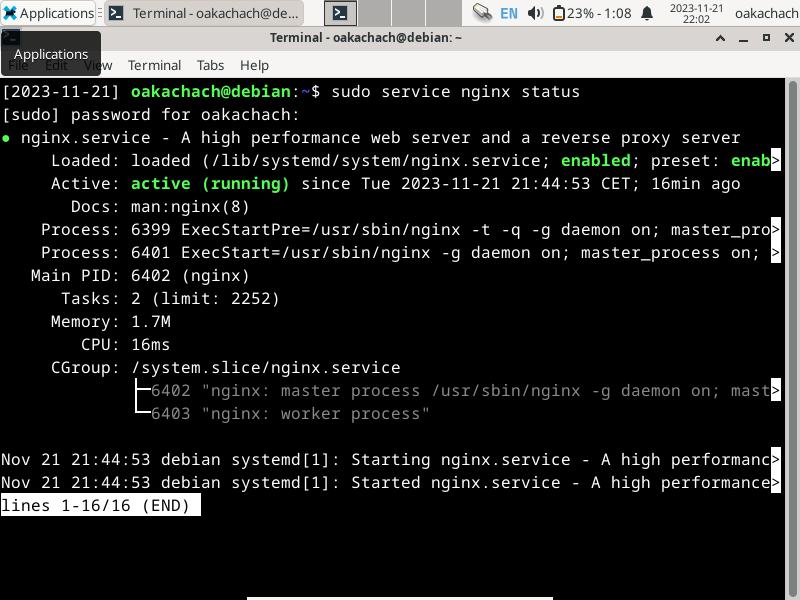
\includegraphics[scale=0.45]{../img/1.png}
\end{center}

\newpage

\subsection{}

\textit{¿En qué dirección IP se está ejecutando el servidor
RTMP? Comprobadlo con el comando ifconfig o con cualquier
otra herramienta similar, mostrándolo mediante una captura
de pantalla.}

\begin{center}
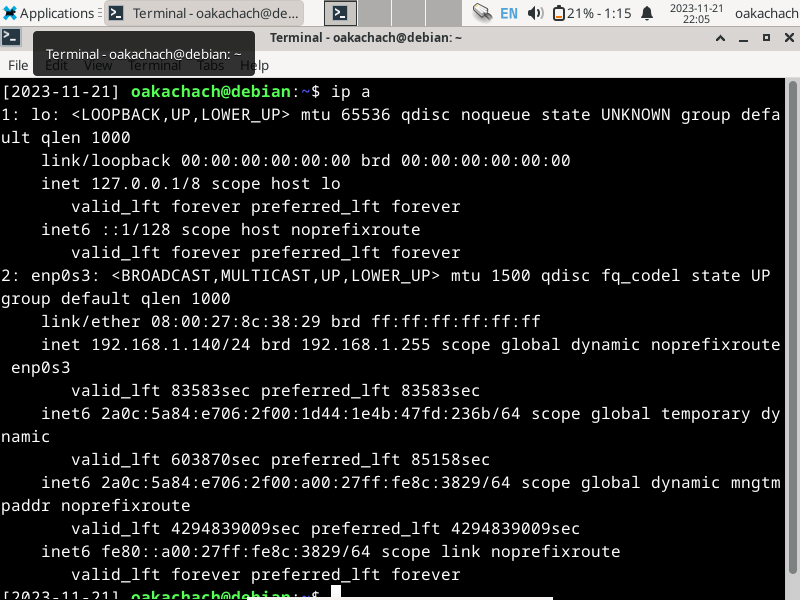
\includegraphics[scale=0.45]{../img/2.png}
\end{center}

\subsection{}

\textit{¿En qué puerto se está ejecutando el servidor RTMP?
¿En qué estado está? Comprobadlo con el comando netstat o
con cualquier otra herramienta similar, mostrándolo mediante
una captura de pantalla.}

\begin{center}
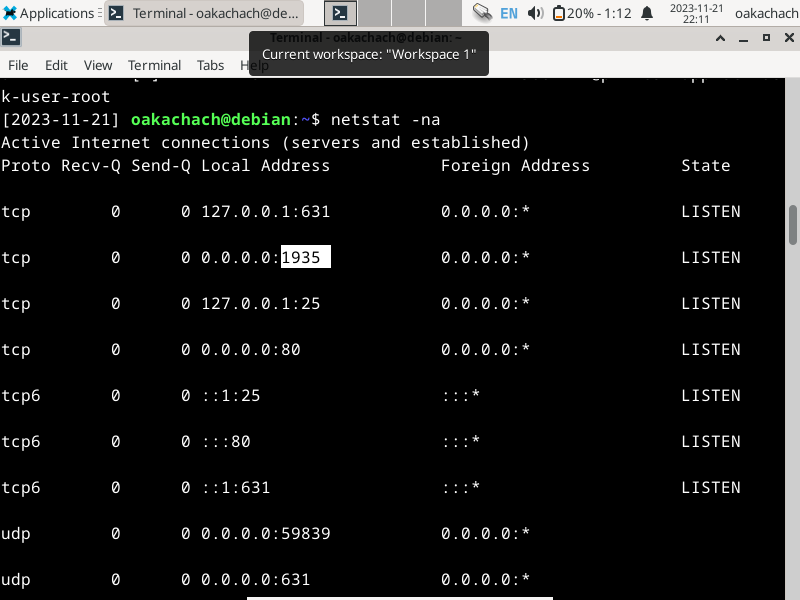
\includegraphics[scale=0.45]{../img/3.png}
\end{center}

\subsection{}

\textit{En cualquier navegador web, introducid la siguiente
URL:}

\begin{center}
``http://\(<\)ip\_de\_tu\_servidor\(>\)''
\end{center}

\textit{Mostrad
mediante una captura de pantalla que el servidor web está
correctamente configurado.}

\begin{center}
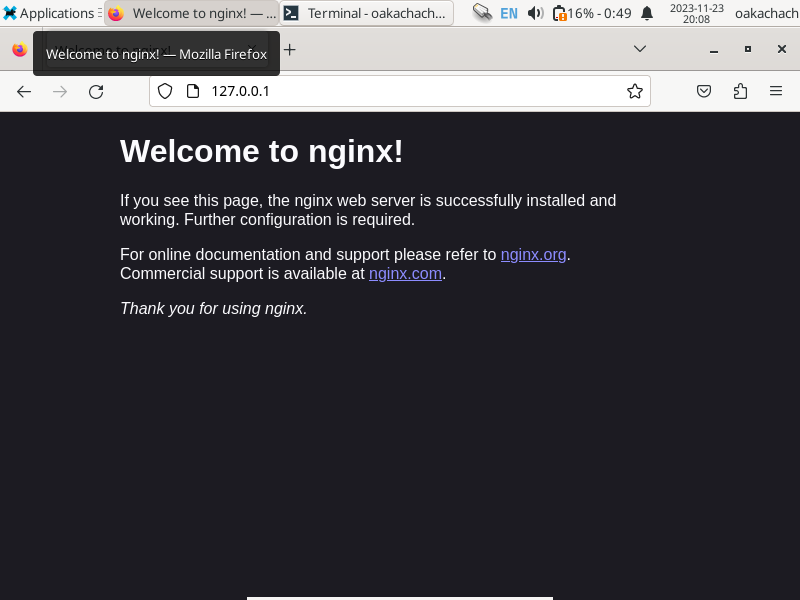
\includegraphics[scale=0.45]{../img/4.png}
\end{center}

\section{Pregunta 2}

\subsection{}

\textit{Explicad qué significan todas las opciones del
comando anterior ffmpeg.}\\

-re: Lee el archivo de entrada al mismo frame rate del
propio archivo.\\

-i: Indica la dirección del archivo origen.\\

-c:v copy: Indica la opción del códec de vídeo, establecida a
``copy'', así que no se producirán operaciones de
decodificado/filtrado/codificado.\\

-c:a aac: Indica la opción del códec de audio, establecida a
``aac''.\\

-ar 44100: Establece la frecuencia de muestreo del audio a
44100 Hz.\\

-ac 1: Establece el número de canales de audio a 1.\\

-f flv: Fuerza el formato de entrada o salida (a flv).\\

-flvflags no\_duration\_filesize: Desactiva la duración y el
tamaño de archivo en los metadatos cuando son iguales a cero
al final del flujo.

\subsection{}

\textit{Explicad por qué en la URL a la que estamos enviando
el vídeo aparecen las palabras live y stream.}\\

Se trata del endpoint al que accedemos para ver los
contenidos de la retransmisión.

\subsection{}

\textit{¿A cuántos frames por segundo se está transmitiendo
el vídeo?}\\

A 30 frames por segundo.

\subsection{}

\textit{Conectaos con VLC o cualquier otro reproductor a la
URL:}

\begin{center}
``rtmp://\(<\)ip\_de\_tu\_servidor\(>\)/live/stream''
\end{center}

\textit{Mientras el vídeo se esté subiendo con el programa de
streaming ffmpeg. Pegad una captura de pantalla donde se vea
que el vídeo se está reproduciendo.}

\begin{center}
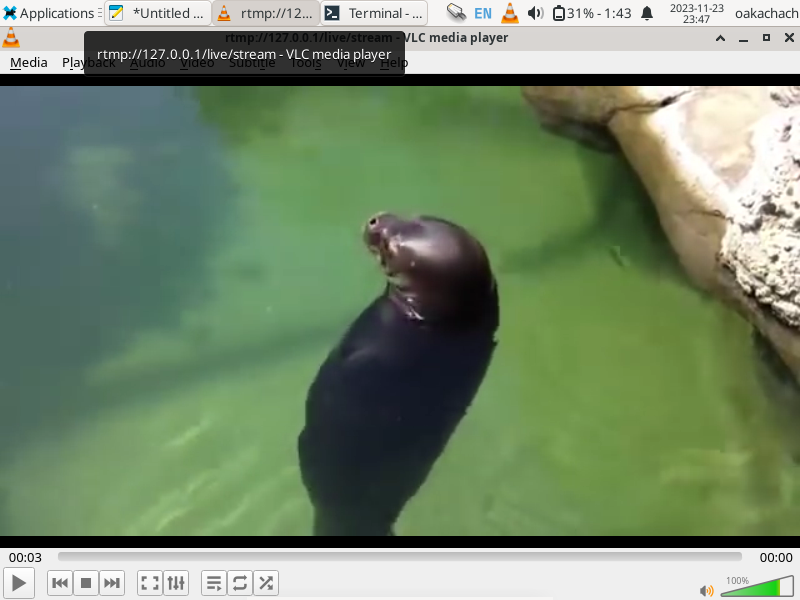
\includegraphics[scale=0.45]{../img/5.png}
\end{center}

\subsection{}

\textit{La emisión terminará cuando el vídeo pare. ¿Qué
habría que hacer para reproducirlo en bucle?}\\

Se deben introducir los argumentos +genpts -stream\_loop. El
primero es para evitar que bajen los frames al reproducir de
nuevo el clip, regenerando el pts desde el principio. El
flag -stream\_loop permite reproducir el vídeo las veces que
queramos.\\

Se debe tener en cuenta que estos argumentos se deben
introducir antes que el -i.

\subsection{}

\textit{¿Cuál es el bitrate medio al que se ha
transmitido?}\\

370 kbits por segundo.

\section{Pregunta 3}

\subsection{}

\textit{Para comprobar que se está transmitiendo el
streaming en tiempo real, conectaos con VLC o similar a la
URL
rtmp://\(<\)ip\_de\_tu\_servidor\(>\)/live/\(<\)usuario\_uoc\(>\).
Mostradlo mediante una captura de pantalla.}

\begin{center}
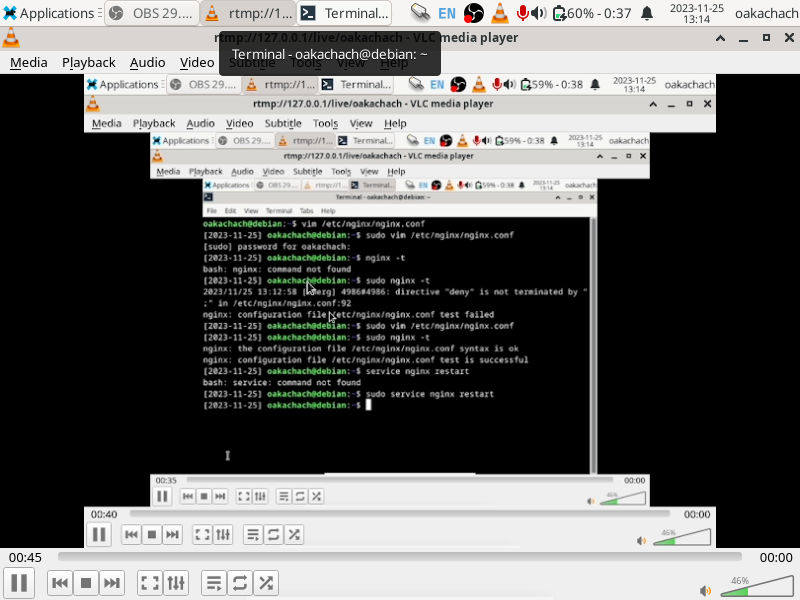
\includegraphics[scale=0.45]{../img/6.png}
\end{center}

\subsection{}

\textit{Realiza acciones de usuario sobre la pantalla donde
estáis ejecutando OBS y fijaos en el streaming que estáis
visualizando con VLC o similar. ¿Qué es lo que estáis
retransmitiendo?}\\

Se está retransmitiendo el contenido de la pantalla que, en
este caso, está siendo mi ratón interactuando con la
interfaz de OBS.

\subsection{}

\textit{Pensad un vídeo a reproducir que contenga como
mínimo tres escenas con varias fuentes. Explicad vuestra
idea y mostrad mediante capturas de pantalla la
configuración de OBS y la reproducción del streaming con
VLC.}\\

Un ejemplo así de complejo que me viene a la mente sería un
típico stream de gaming, donde el/la usuario/a está
retransmitiendo, por una parte, el contenido del juego, su
cámara y el output del chat, en tiempo real.\\

De las posibles escenas que podría tener, tenemos:

\begin{enumerate}
\item La escena principal, donde el/la usuario/a tiene el
juego en pantalla completa, el chat en una esquina, y la
camara en otra. Estos dos últimos ocupan el mínimo espacio
posible, puesto que queremos mantener el foco en el
contenido del videojuego que se está retransmitiendo.
\item La escena de ``Just chatting'', que es cuando el/la
usuario/a no está jugando a nada e interactúa con el chat.
En esta escena, la cámara es la que ocupa toda la pantalla,
teniendo el chat en una esquina, como antes. El juego no se
visualiza, puesto que o no se está ejecutando, o no hace
falta mostrarlo porque no es de interés actualmente.
\item La escena de ``Enseguida vuelvo''. Esta escena tiene
únicamente el chat, pero no aparece ni el contenido del
juego, ni la cámara del/la usuario/a. Esto es debido a que,
por algun motivo, el/la ``streamer'' está ausente del lugar
y no se está mostrando ningún tipo de contenido.
\end{enumerate}

Debido a las limitaciones técnicas que tenemos al trabajar
en una máquina virtual con tan poca RAM, sin la posibilidad
de transmitir videojuegos o el output de una webcam, se
mostrarán como fuentes diferentes imágenes, con el título
del contenido que representan:

\newpage

Escena principal:

\begin{center}

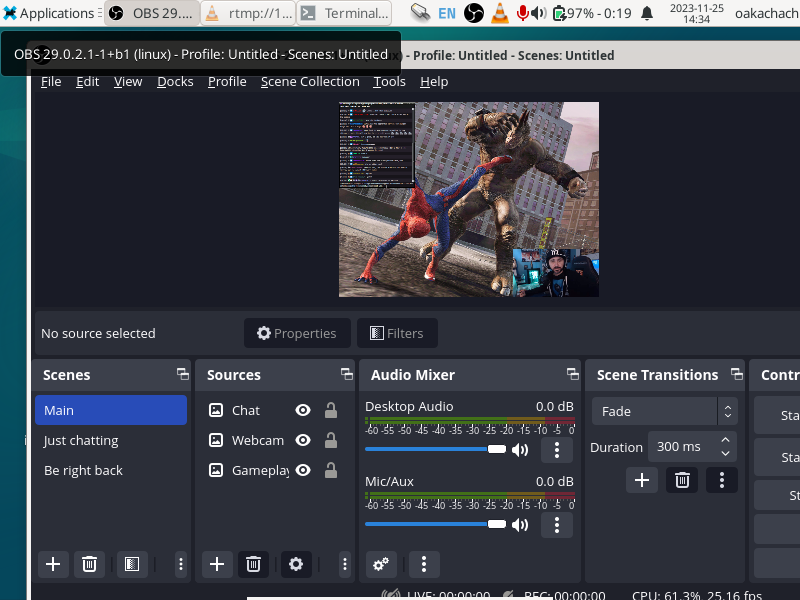
\includegraphics[width=10cm]{../img/7.png}
\end{center}

Escena de ``Just chatting'':

\begin{center}
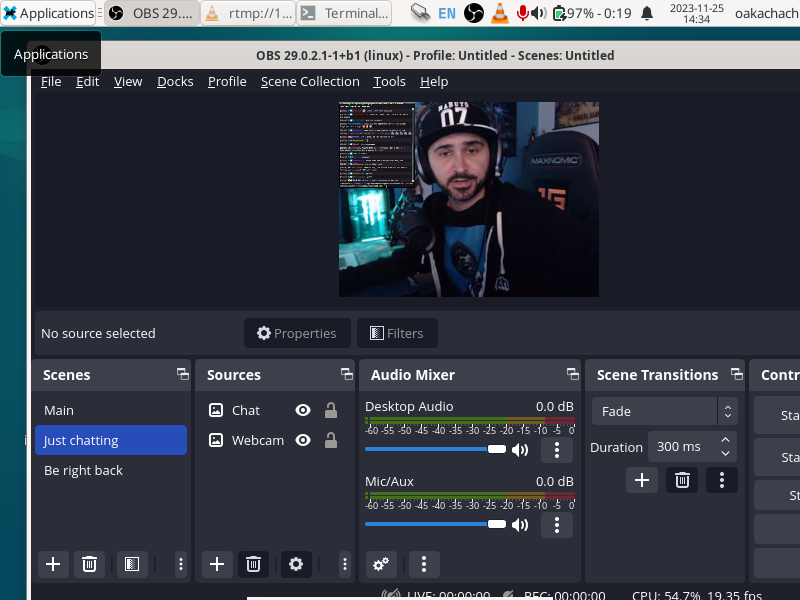
\includegraphics[width=10cm]{../img/8.png}
\end{center}

\newpage

Escena de ``Enseguida vuelvo'':
\begin{center}
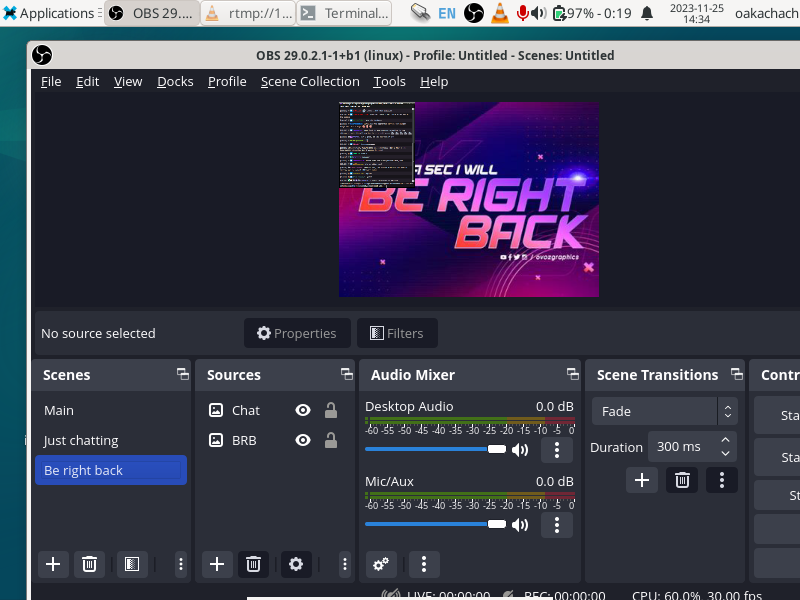
\includegraphics[width=9cm]{../img/9.png}
\end{center}

\subsection{}

\textit{Abrid el programa Wireshark como root antes de
empezar la transmisión del streaming en vivo. Pegad una
captura de pantalla donde se vea el tráfico RTMP que se ha
generado. Podéis filtrar por protocolo RTMP para ver solo
esta interacción. Explicad razonadamente, paquete a paquete,
la primera fase de establecimiento de la conexión
(handshake) con la negociación de parámetros (hasta los
paquetes audio/video data).}\\

\begin{center}
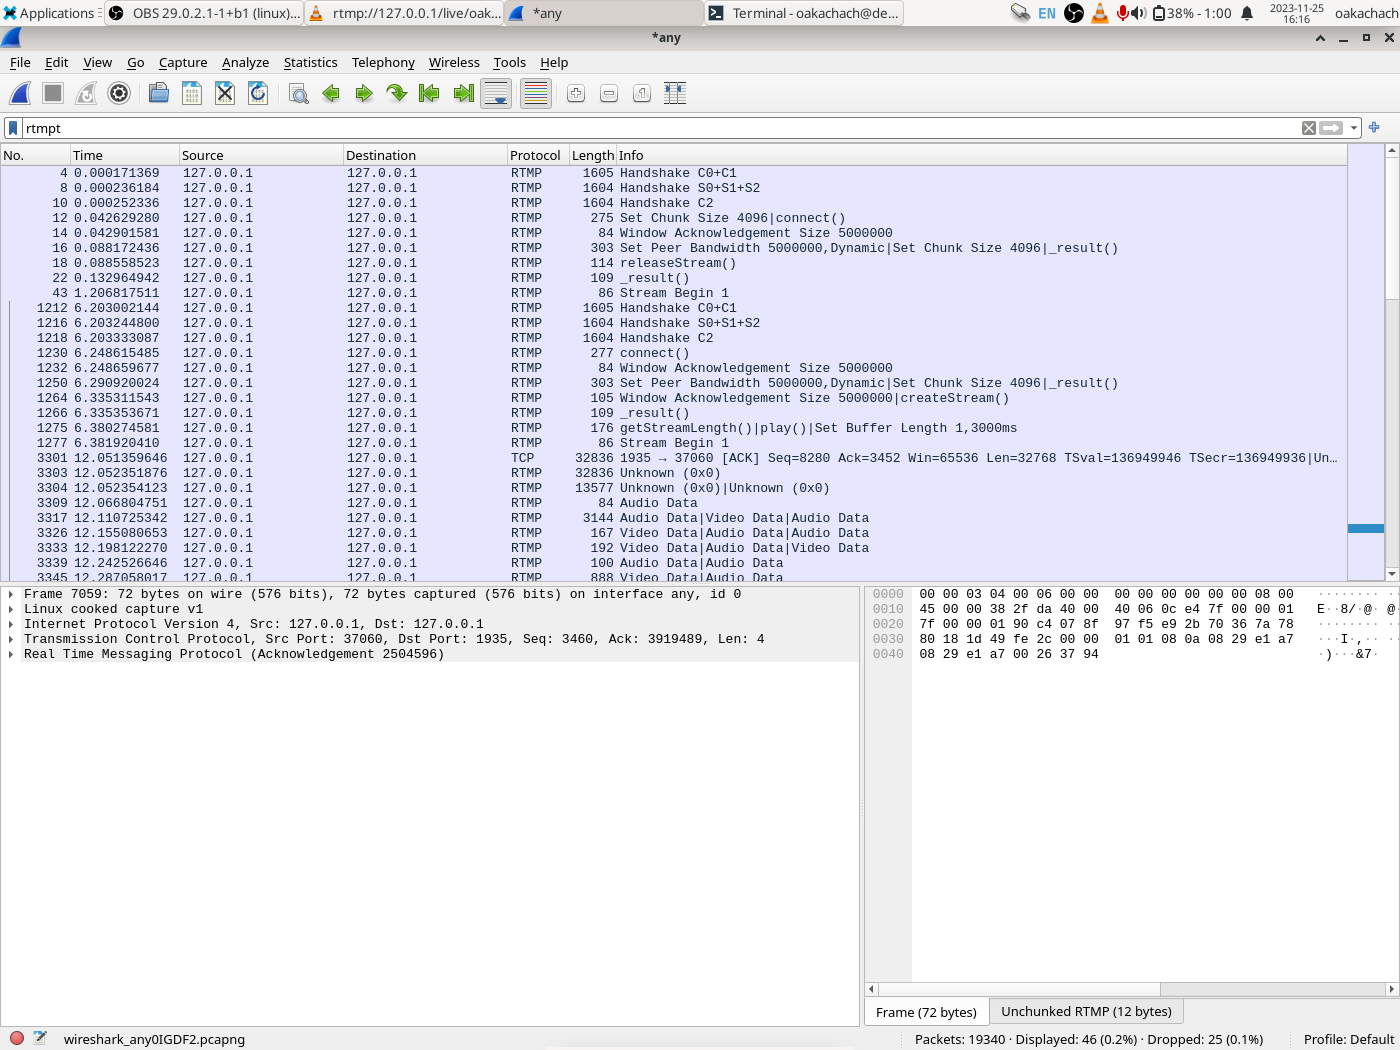
\includegraphics[width=10cm]{../img/10.png}
\end{center}

La primera fase de establecimiento de la conexión
(handshake) ocurre en los paquetes 4, 8 y 10.\\

En el paquete 4, enviamos datos del handshake del puerto
53316, al 1935, que es el que está configurado para nuestro
servidor RTMP.\\

El siguiente paquete, el 8, envia datos del handshake del
puerto 1935, al 53316. La cantidad es la misma a excepción
de un byte.\\

El siguiente paquete, el 10, envia datos, de nuevo, del
puerto 53316 al 1935, con la misma cantidad de bytes de
vuelta, con tal de confirmar que la conexión entre cliente y
servidor se ha realizado correctamente.\\

Los paquetes 12, 14 y 16 son los encargados de la
negociación de parámetros. En el primero, el 12, se
establece el tamaño de los chunks a 4096 bytes, como tenemos
indicado en nuestro nginx.conf. También se envía el comando
connect(), en el cual se indica la url de nuestro stream,
además de otros parámetros.\\

Seguido de ello, en el paquete 14, se establece el tamaño de
la ventana de reconocimiento, con tal de evitar congestiones
entre servidor y cliente.\\

Por último, en el paquete 16, se envía, del puerto 1935 al
53316, el valor de ancho de banda, igual a la ventana de
reconocimiento enviada anteriormente, y se establece el tipo
de límite a ``dinámico''. También se ejecuta el comando
result(), donde podemos ver que la conexión se ha realizado
correctamente. Esto viene como respuesta del paquete 16,
donde se envió el comando connect().\\

En el paquete 18, se ejecuta el comando releaseStream(), en
el que se envía como parámetros nuestra clave de streaming.
Y en el paquete 22 el servidor nos devuelve la respuesta
con el comando result().\\

En el paquete 43, comienza la retransmisión, donde se envía
el paquete del puerto 1935, al 52040, justo cuando entramos
en la URL de nuestro stream, a través de VLC.\\

Los paquetes 1212, 1216 y 1218 sirven para enviar datos del
handshake, de la misma manera que ocurrió al inicio de la
ejecución de la retransmisión.\\

Desde el puerto 37060, al puerto 1935, en el paquete 1230,
se envía el comando connect(), con nuestra versión de flash
y la URL a la que nos queremos conectar. Enviamos
información de nuestros códecs de audio y de video, entre
otras características.\\

Los paquetes 1232, 1250 y 1264 sirven para establecer la
negociación de parámetros y en el paquete 1266 el servidor
nos envía el comando result(), con la información
resultante.\\

El paquete 1275 es para enviar al servidor RTMP el comando
getStreamLength() y play() y para establecer el tamaño del
buffer a 1.3ms.\\

El servidor envía el mensaje Stream Begin de vuelta en el
paquete 1277.\\

A partir del paquete 3309, comienzan el flujo de paquetes
Audio y Video data.

\subsection{}

\textit{Parad la reproducción del streaming en VLC y OBS.
¿Qué paquetes se generan en Wireshark? Explicad brevemente
la interacción que observéis, ejemplificándolo con alguna
captura de pantalla.}

\begin{figure}[!htbp]
\begin{center}
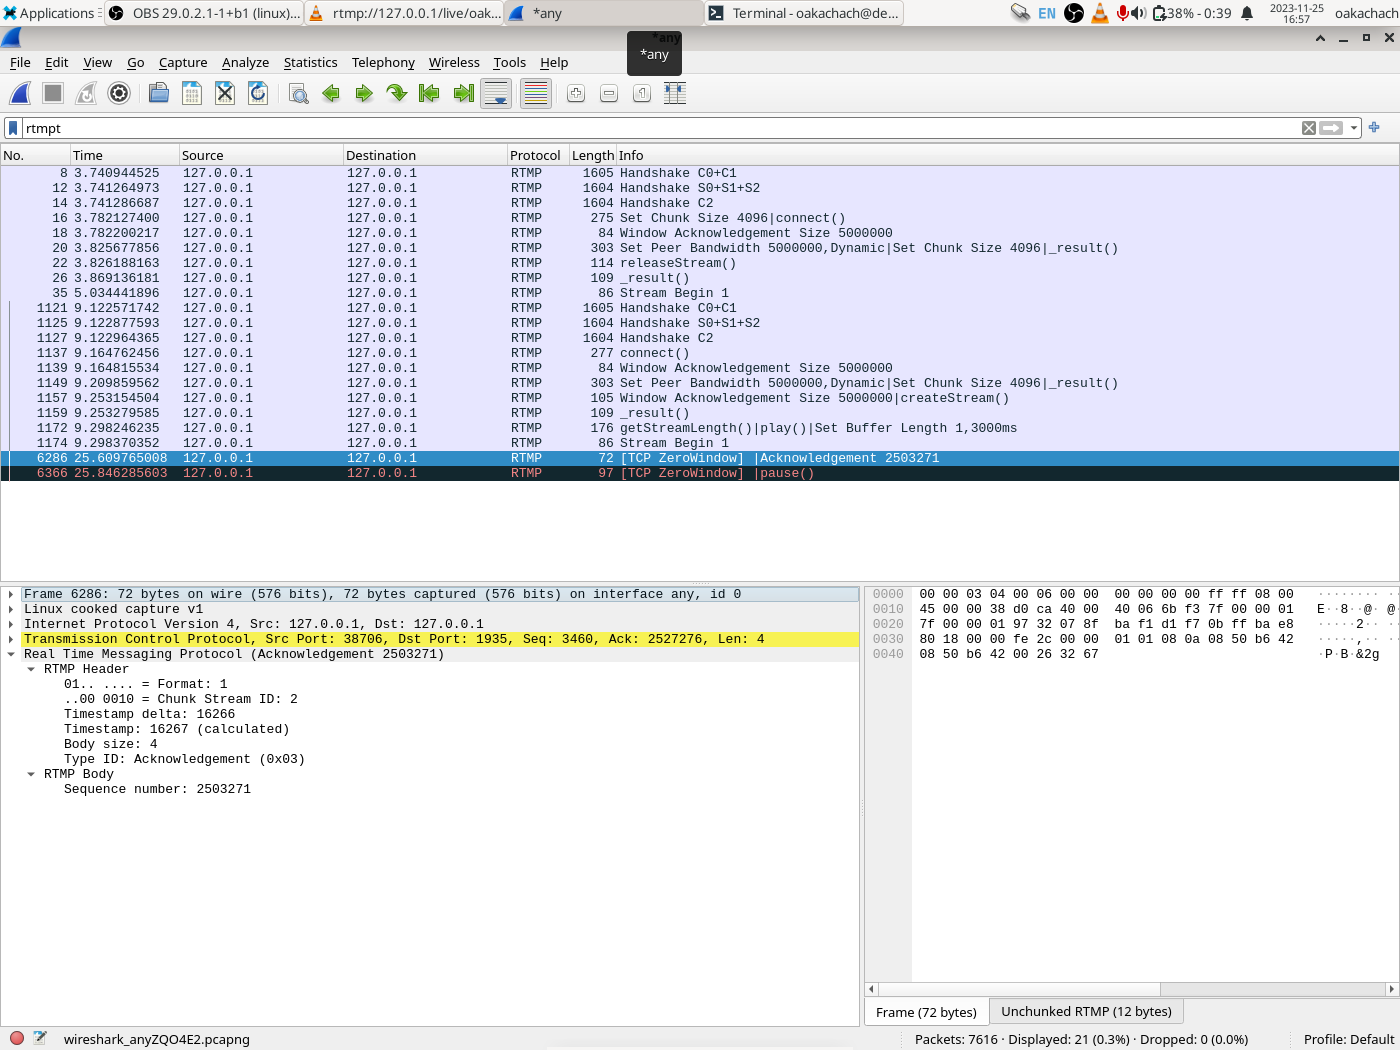
\includegraphics[width=10cm]{../img/11.png}
\caption{Captura de pantalla de Wireshark}
\end{center}
\end{figure}

En el paquete 6286, el puerto 38706 envía al servidor RTMP
el número de secuencia 2503271. Esto ocurre cuando pausamos
la retransmisión desde VLC.\\

Por último, en el paquete 6366, el puerto 38706 envía al
servidor RTMP el comando pause(). Esto ocurre cuando
pausamos la retransmisión desde OBS.

\newpage

\section{Pregunta 4}

Captura de pantalla de la página de estadísticas:

\begin{center}
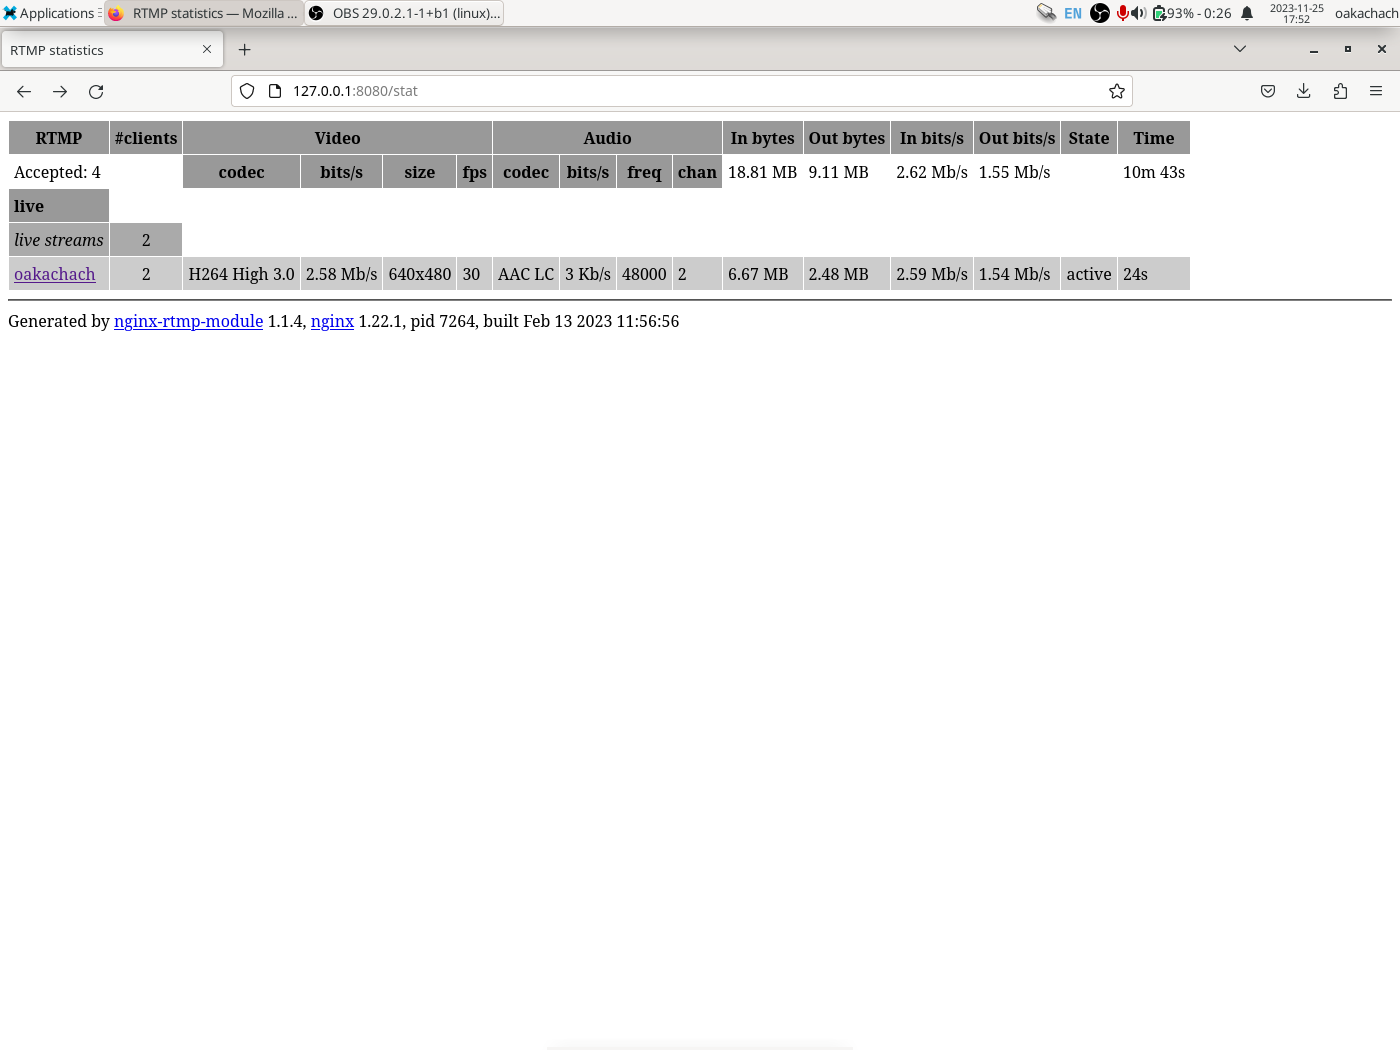
\includegraphics[width=10cm]{../img/12.png}
\end{center}

\subsection{}

\textit{En relación con la transmisión de audio, indicad:}

\subsubsection{}

\textit{¿Cuál es el códec que se está usando?}\\

Se está utilizando AAC LC como códec de audio.

\subsubsection{}

\textit{¿Cuál es el bitrate?}\\

El bitrate es de 3 Kb/s.

\subsubsection{}

\textit{¿Cuál es la frecuencia?}\\

La frecuencia es de 48000 Hz.

\subsubsection{}

\textit{¿Y el canal?}\\

El canal utilizado es el 2.

\subsection{}

\textit{En relación con la transmisión de vídeo, indicad:}

\subsubsection{}

\textit{¿Cuál es el códec que se está usando?}\\

Se está utilizando H264 High 3.0 como códec de vídeo.

\subsubsection{}

\textit{¿Cuál es el bitrate?}\\

El bitrate es de 2.58 Mb/s.

\subsubsection{}

\textit{¿A qué resolución se está transmitiendo?}\\

Se está retransmitiendo a una resolución de 640x480 píxeles.

\subsubsection{}

\textit{¿A cuántos frames por segundo?}\\

Se está retransmitiendo a 30 frames por segundo.

\section{Pregunta 5}

\subsection{}

\textit{Explicad todos los parámetros de configuración de RTMP que
habéis añadido en los dos ficheros de configuración
anteriores.}\\

\textbf{hls on:} Activa el streaming en HLS para el servidor
determinado.\\

\textbf{hls\_path /var/www/html/stream/hls:} Establece el directorio
de los archivos de vídeo de HLS y sus playlists.\\

\textbf{hls\_fragment 3:} Define la longitud de fragmento
predeterminada a 3 segundos.\\

\textbf{hls\_playlist\_length 60:} Define la longitud de la playlist
a 60 segundos.\\

\textbf{dash on:} Activa el streaming en DASH para el servidor
determinado.\\

\textbf{dash\_path /var/www/html/stream/dash:} Establece el directorio de los archivos de vídeo
de DASH y sus playlists.\\

\textbf{server.listen 8088:} Establece el puerto que utilizará el
servidor.\\

\textbf{server.location /:} Establece la ubicación que nginx
utilizará para administrar las peticiones del servidor.\\

\textbf{server.location.add\_header
Access-Control-Allow-Origin *:}
Añade el campo especificado a una cabecera de respuesta,
siempre y cuando no sea un error.\\

\textbf{server.location.root /var/www/html/stream:} Establece la
ubicación raíz del servidor.\\

\textbf{types.application/dash+xml mpd:} Establece el formato de
salida del vídeo para el protocolo DASH.

\subsection{}

\textit{Comprobad con el comando netstat o con cualquier otra
herramienta similar los servicios que se han configurado,
mostrándolo mediante una captura de pantalla.}

\begin{center}
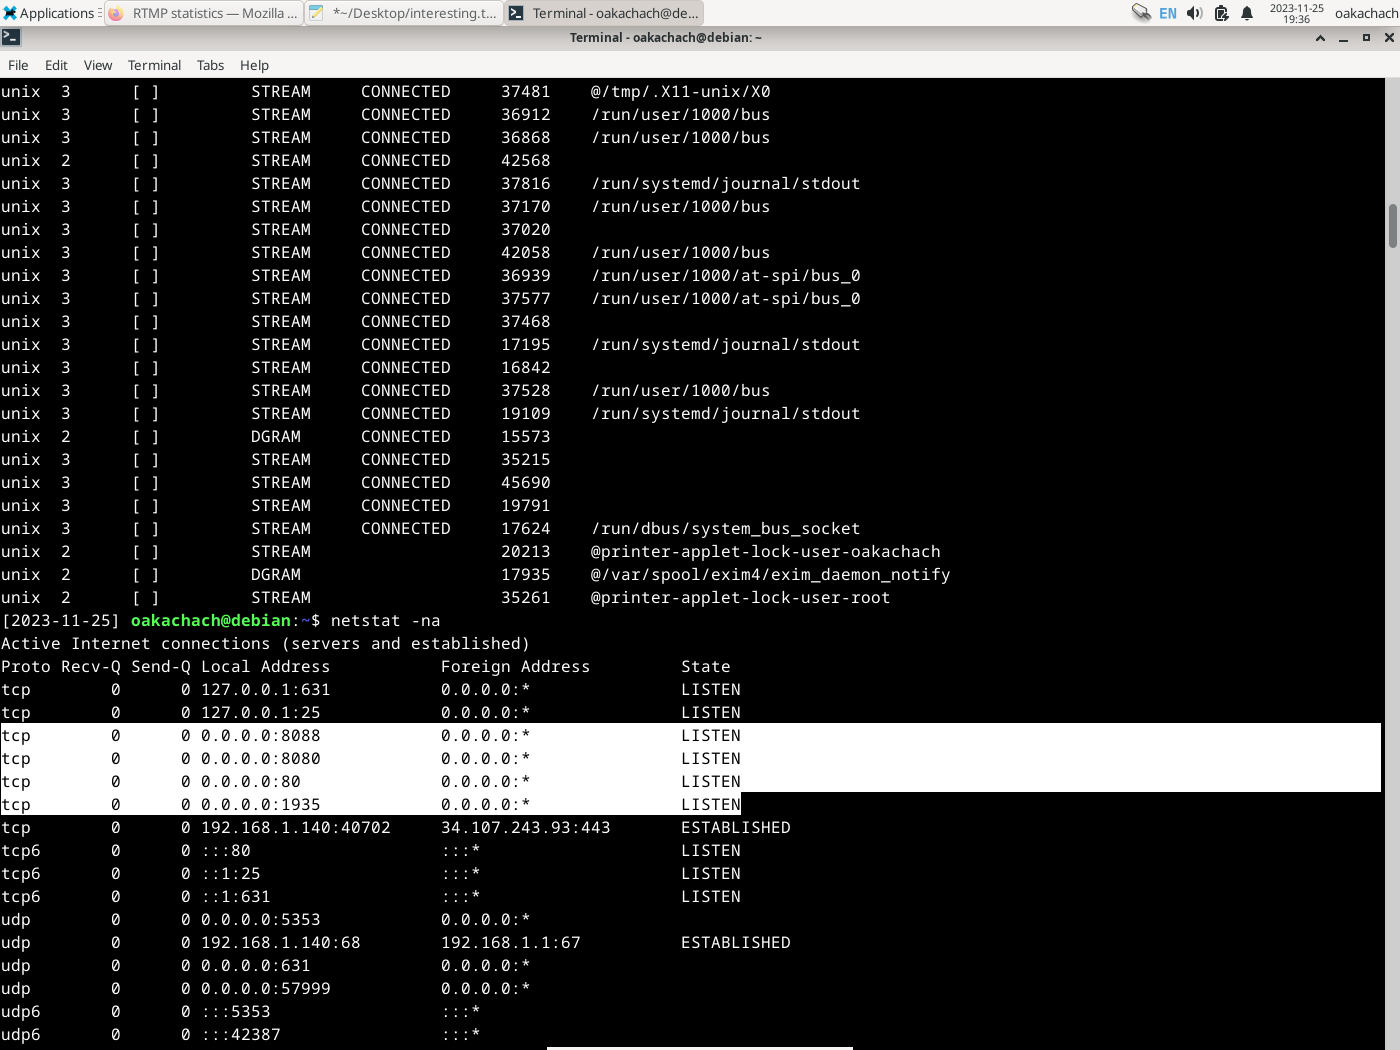
\includegraphics[width=10cm]{../img/13.png}
\end{center}

\subsection{}

\textit{Conectaos con VLC a:}

\begin{center}
``http://\(<\)ip\_servidor\(>\):8088/hls/stream.m3u8''
\end{center}

\textit{Y comprobad que podéis ver el stream HLS por HTTP. Pegad una
captura de pantalla.}

\begin{center}
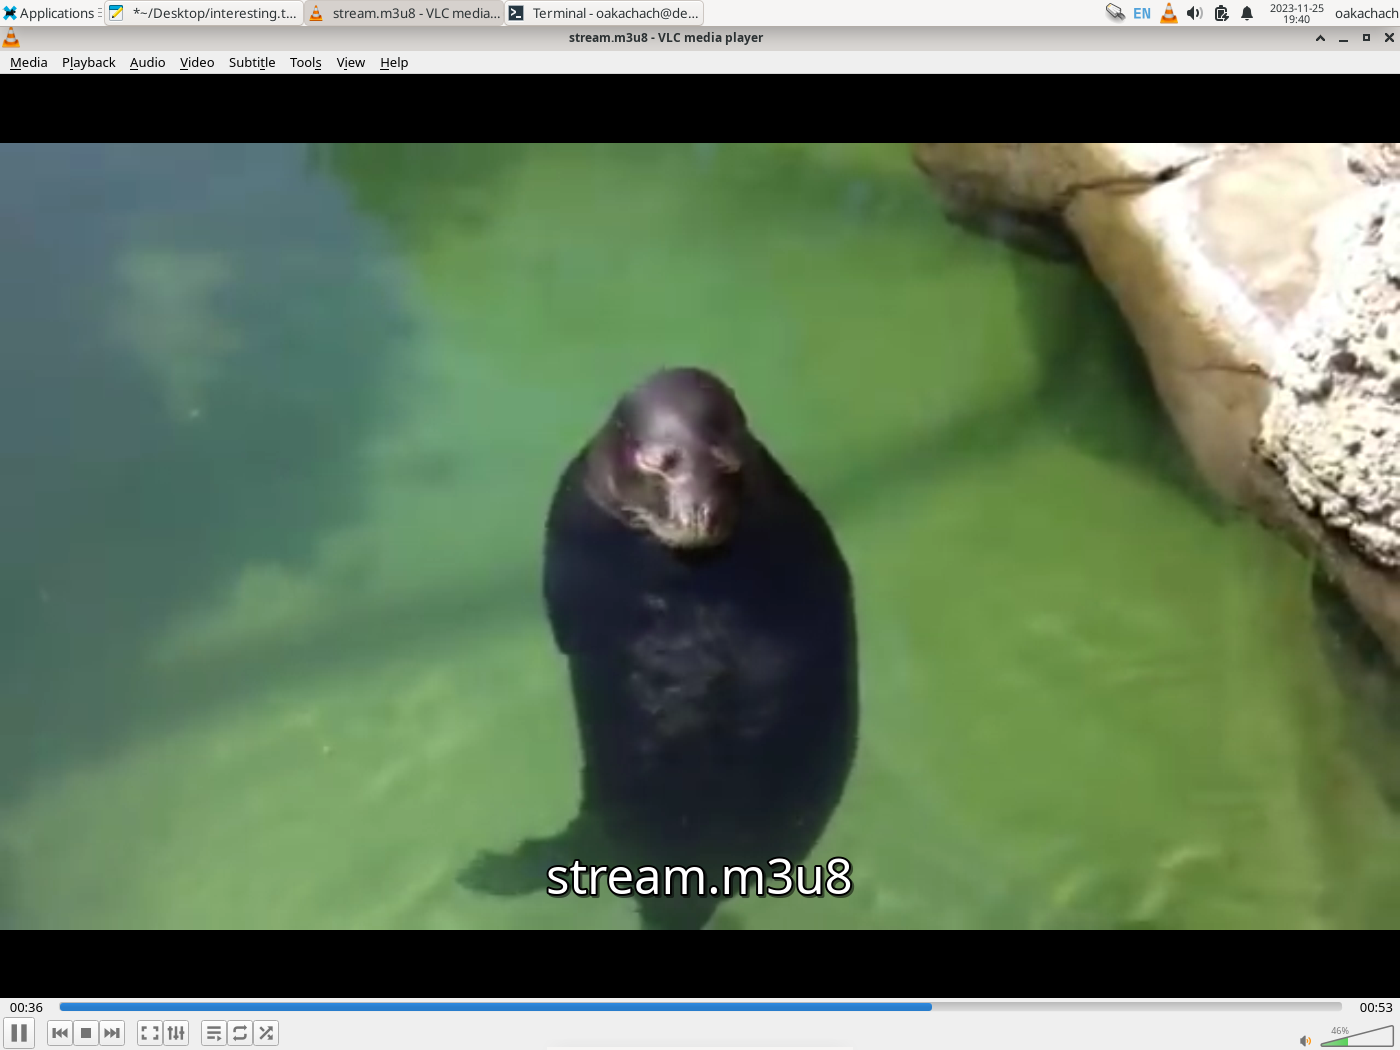
\includegraphics[width=10cm]{../img/14.png}
\end{center}

\newpage

\subsection{}

\textit{Abrid el Wireshark y comprobad cómo se transmite el
streaming HLS. Podéis filtrar por puerto para
visualizar los paquetes que nos interesan. Analizad la
interacción que se da, desde el inicio de la reproducción
hasta su paro. Podéis pegar capturas de pantalla y
explicarlas. ¿En qué campo vemos que el streaming es HLS?}\\

\begin{center}
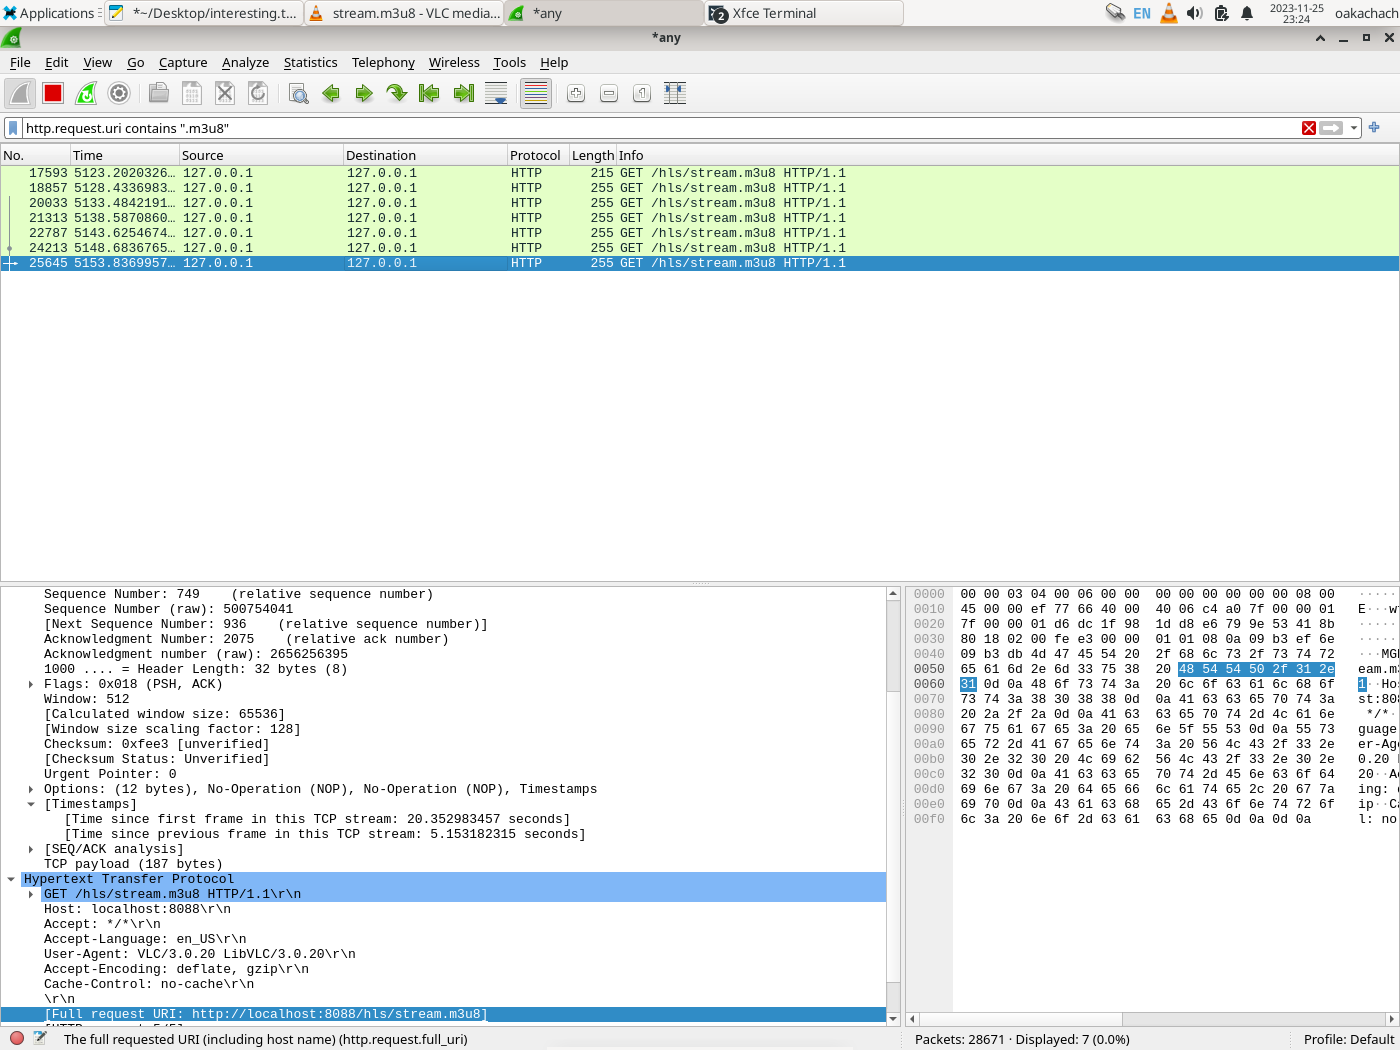
\includegraphics[width=10cm]{../img/16.png}
\end{center}

Para poder determinar que el streaming es HLS, se realiza
un filtro donde la uri de las requests HTTP de los paquetes
contenga la extensión ``.m3u8'', que es la utilizada por
HLS.\\

Dentro del paquete, en el campo Full Request URI, podemos
ver la dirección que usa para conectarse es la misma que la
que hemos introducido en VLC.

\newpage

\subsection{}

\textit{Conectaos con VLC a:}

\begin{center}
``http://\(<\)ip\_servidor\(>\):8088/dash/stream.mpd''
\end{center}

\textit{Y comprobad que podéis ver el stream DASH por HTTP. Pegad
una captura de pantalla.}

\begin{center}
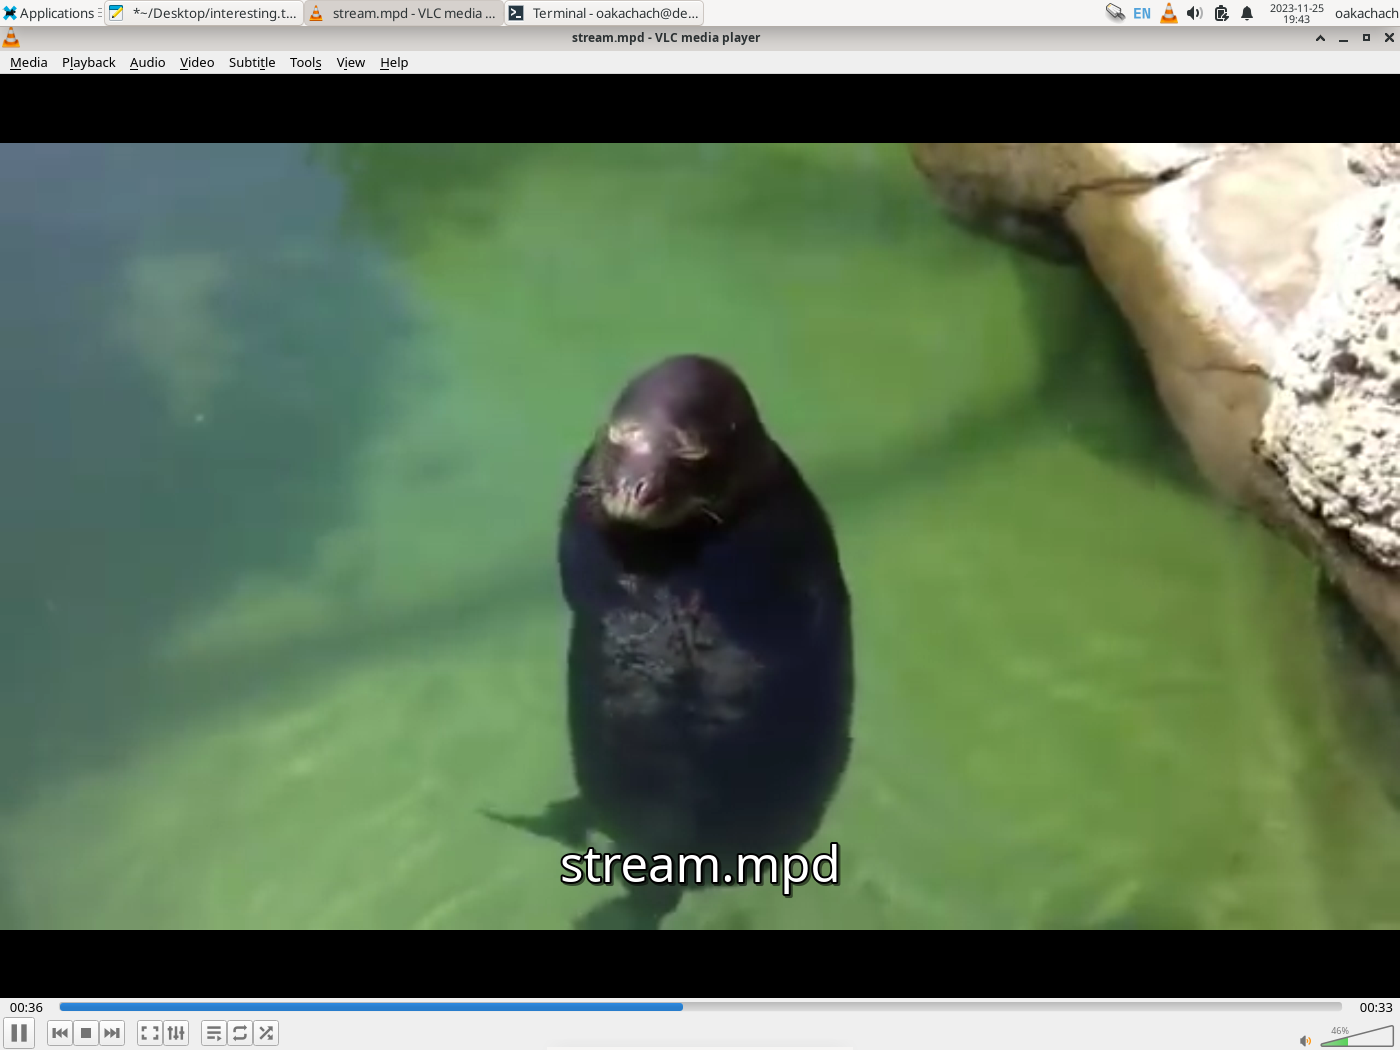
\includegraphics[width=9cm]{../img/15.png}
\end{center}

\newpage

\subsection{}

\textit{Abrid el Wireshark y comprobad cómo se transmite el
streaming DASH. Podéis filtrar por puerto para visualizar
los paquetes que nos interesan. Analizad la interacción que
se da, desde el inicio de la reproducción hasta su paro.
Podéis pegar capturas de pantalla y explicarlas. ¿En qué
campo vemos que el \textit{streaming} es DASH?}

\begin{center}
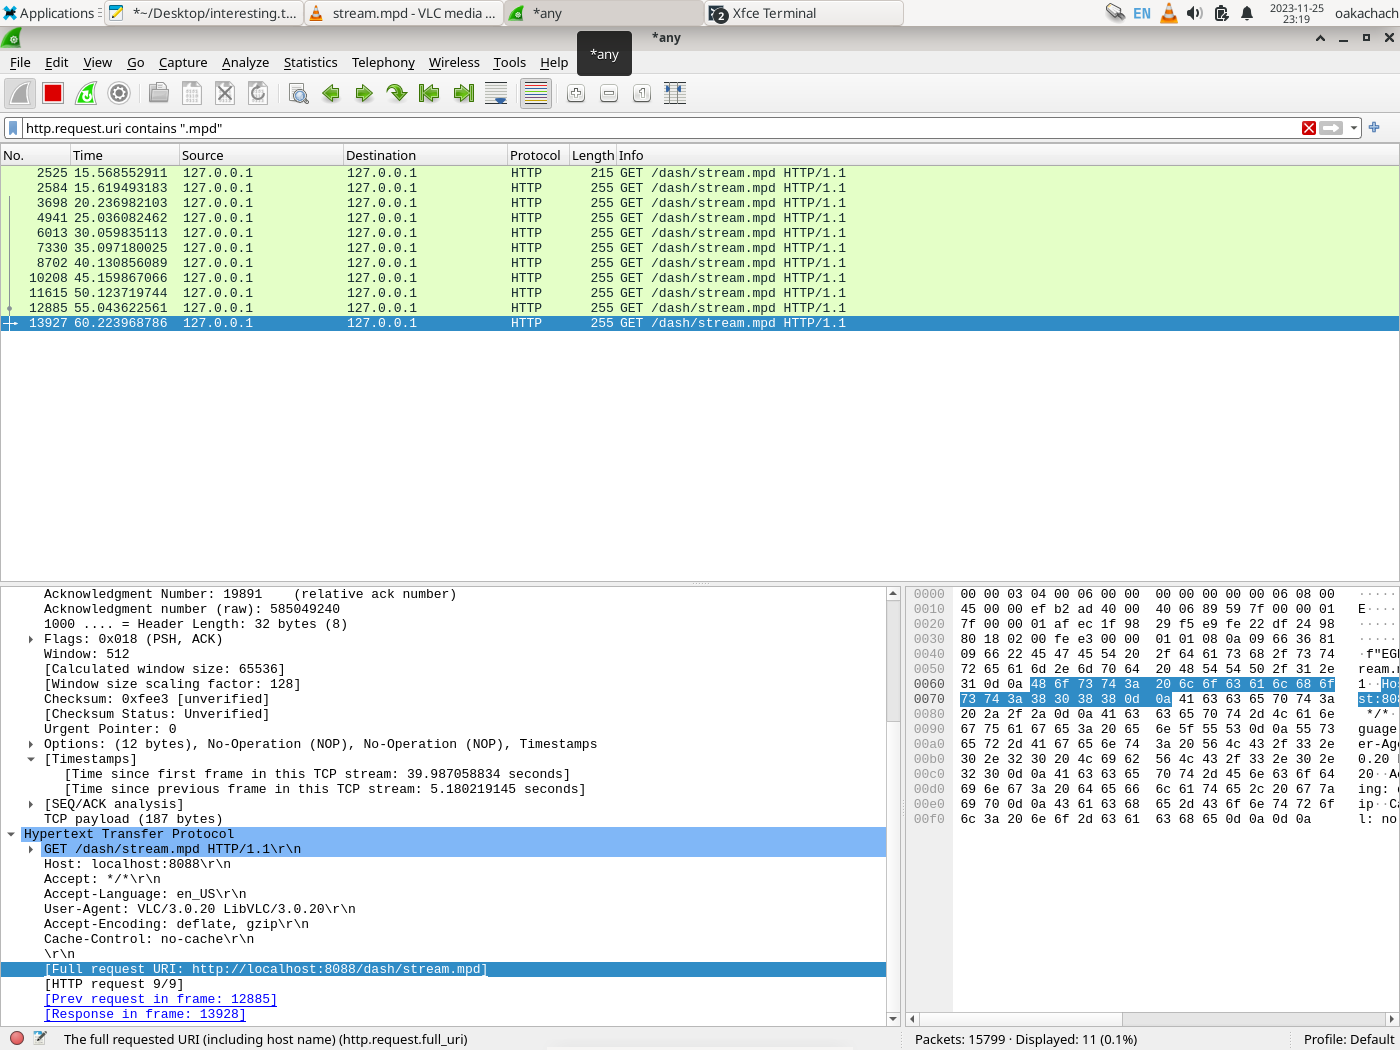
\includegraphics[width=9cm]{../img/17.png}
\end{center}

Para poder determinar que el streaming es DASH, se realiza
un filtro donde la uri de las requests HTTP de los paquetes
contenga la extensión ``.mpd'', que es la utilizada por
DASH.\\

Dentro del paquete, en el campo Full Reuqest URI, podemos
ver la dirección que usa para conectarse es la misma que la
que hemos introducido en VLC.

\subsection{}

\textit{¿Hay diferencias entre HLS y DASH? Comentadlas.}\\

Antiguamente, HLS era un protocolo que se utilizaba para
retransmitir contenido através de HTTP a dispositivos de
Apple. En cambio, DASH es un protocolo más abierto e
independiente, que se ha convertido en un estándar
internacional, a diferencia de HLS, que fue desarrollado por
Apple.\\

DASH permite el uso de cualquier estándar de codificación,
mientras que HLS requiere el uso de H.264 o H.265.\\

Por último, HLS tiene una longitud de segmento de 6
segundos, aunque se puede ajustar, mientras que los
segmentos de DASH son entre 2 y 10 segundos.\\

\begin{thebibliography}{X}
\item \textit{ffmpeg Documentation.} (n.d.).
https://ffmpeg.org/ffmpeg.html\\
\item Wikipedia contributors. (2023, October 17).
\textit{Chunked transfer encoding.} Wikipedia.
https://en.wikipedia.org/wiki/Chunked\_transfer\_encoding\\
\item IONOS editorial team. (2023, March 3). NGINX Tutorial
- \textit{Commands and configurations.} IONOS Digital Guide. https://www.ionos.com/digitalguide/server/configuration/nginx-tutorial-getting-started-with-nginxconf/
\item \textit{nginx news.} (n.d.). https://nginx.org/\\
\item \textit{What is MPEG-DASH} (n.d.). https://www.cloudflare.com/learning/video/what-is-mpeg-dash/
\end{thebibliography}

\end{document}
